\documentclass[11pt,a4paper]{article}
\usepackage[utf8x]{inputenc}
\usepackage[czech]{babel}
\usepackage[IL2]{fontenc}
\usepackage{amsmath}
\usepackage{amsfonts}
\usepackage{amssymb}
\usepackage{tabularx}
\usepackage{graphics}
\usepackage[left=2cm,right=2cm,top=3cm,bottom=3cm]{geometry}
\author{Viktor Jančík}

\usepackage{times}
\usepackage[]{verbatim}

\usepackage{multirow}
\usepackage[ruled,vlined,linesnumbered]{algorithm2e}


\begin{document}
\begin{titlepage}

% \vspace*{1cm}
\begin{figure}[!h]
  \centering
  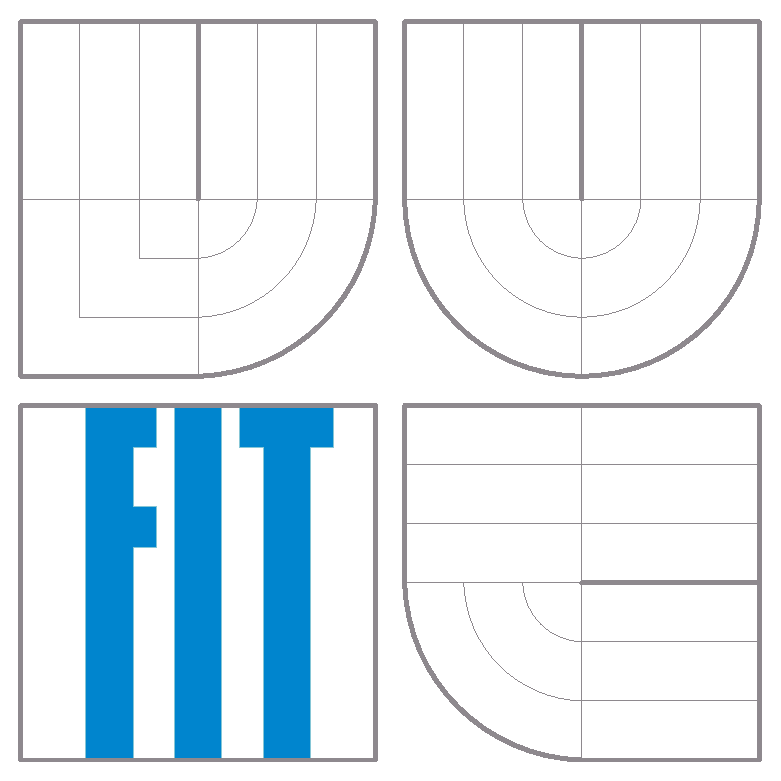
\includegraphics[height=5cm]{img/logo}
\end{figure}

\vfill

\begin{center}
\begin{Large}
Téoria obvodov\\
\end{Large}
\bigskip
\begin{Huge}
Semestrálny projekt\\
\end{Huge}
\end{center}

\vfill

\begin{center}
\begin{Large}
\today
\end{Large}
\end{center}

\vfill

\begin{flushleft}
\begin{large}
\begin{tabular}{ll}
Autor: 
 & Viktor Jančík, \url{xjanci09@stud.fit.vutbr.cz} \\
 & Fakulta Informačních Technologií \\
 & Vysoké Učení Technické v~Brně \\
\end{tabular}
\end{large}
\end{flushleft}
\end{titlepage}


\section{Úvodní strana}

Název práce umístěte do zlatého řezu a nezapomeňte uvést dnešní datum a vaše jméno a příjmení.

\section{Tabulky}

Pro sázení tabulek můžeme použít buď prostředí \verb|tabbing| nebo prostředí \verb|tabular|.

\subsection{Prostředí tabbing}

Při použití \verb|tabbing| vypadá tabulka následovně:

\begin{tabbing}
	Vodni melouny \quad \= Cena \quad \= Mnozstvi \kill    
    \textbf{	Ovoce} \> \textbf{Cena} \> \textbf{Množství} \\
    Jablka \> 25,90 \> 3 kg \\
    Hrušky \> 27,40 \> 2,5 kg \\
    Vodní melouny \> 35,-- \> 1 kus \\
\end{tabbing}

Toto prostředí se dá také použít pro sázení algoritmů, ovšem vhodnější je použiť prostředí \verb|algorithm| nebo \verb|algorithm2e| (viz sekce \ref{sec3}).

\subsection{Prostředí tabular}

Další možností, jak vytvořit tabulku, je použít prostředí \verb|tabular|. tabulky pak budou vypadat takto\footnote{Kdyby byl problem s \texttt{cline}, zkuste se podívat třeba sem: http://www.abclinuxu.cz/tex/poradna/show/325037.}:

\begin{table}[h]
\catcode`\-=12
\centering
\begin{tabular}{|c|c|c|}
 \hline
 & \multicolumn{2}{c|}{\textbf{Cena}} \\ \cline{2-3}
 \textbf{Měna} & \textbf{nákup} &  \textbf{prodej} \\
 \hline
 EUR & 27,34 & 27,42 \\
 GBP & 33,09 & 32,21 \\
 USD & 19,87 & 19,95 \\
 \hline
\end{tabular}
\caption{Tabulka kurzů k dnešnímu dni}
\end{table}

\begin{table}[!htb]
\catcode`\-=12
\centering

\begin{tabular}{cccc}
\begin{tabular}{|c|c|}
 \hline
 \textit{A} & $\neg$\textit{A} \\ \cline{1-2}
 \textbf{P} & N \\ \cline{1-2}
 \textbf{O} & O \\ \cline{1-2}
 \textbf{X} & X \\ \cline{1-2}
 \textbf{N} & P \\
 \hline
\end{tabular}

\begin{tabular}{|c|c|c|c|c|c|}
 \hline
 \multicolumn{2}{|c|}{ \multirow{2}{*}{A $\wedge$ B} } & \multicolumn{4}{c|}{\textit{B}} \\ \cline{3-6}
 \multicolumn{2}{|c|}{} & \textbf{P} & \textbf{O} & \textbf{X} & \textbf{N} \\ \cline{1-6}
 \multirow{4}{*}{A} & \textbf{P} & P & O & X & N \\ \cline{2-6}
 & \textbf{O} & O & O & N & N \\ \cline{2-6}
 & \textbf{X} & X & N & X & N \\ \cline{2-6}
 & \textbf{N} & N & N & N & N \\
 \hline
\end{tabular}

\begin{tabular}{|c|c|c|c|c|c|}
 \hline
 \multicolumn{2}{|c|}{ \multirow{2}{*}{A $\vee$ B} } & \multicolumn{4}{c|}{\textit{B}} \\ \cline{3-6}
 \multicolumn{2}{|c|}{} & \textbf{P} & \textbf{O} & \textbf{X} & \textbf{N} \\ \cline{1-6}
 \multirow{4}{*}{A} & \textbf{P} & P & P & P & P \\ \cline{2-6}
 & \textbf{O} & P & O & P & O \\ \cline{2-6}
 & \textbf{X} & P & P & X & X \\ \cline{2-6}
 & \textbf{N} & P & O & X & N \\
 \hline
\end{tabular}

\begin{tabular}{|c|c|c|c|c|c|}
 \hline
 \multicolumn{2}{|c|}{ \multirow{2}{*}{A $\rightarrow$ B} } & \multicolumn{4}{c|}{\textit{B}} \\ \cline{3-6}
 \multicolumn{2}{|c|}{} & \textbf{P} & \textbf{O} & \textbf{X} & \textbf{N} \\ \cline{1-6}
 \multirow{4}{*}{A} & \textbf{P} & P & O & X & N \\ \cline{2-6}
 & \textbf{O} & P & O & P & O \\ \cline{2-6}
 & \textbf{X} & P & P & X & X \\ \cline{2-6}
 & \textbf{N} & P & P & P & P \\
 \hline
\end{tabular}
\end{tabular}
\caption{Protože Kleeneho trojhodnotová logika je už je "zastaralá", uvádíme si zde příklad čtyřhodnotové logiky}
\end{table}

\section{Algoritmy}\label{sec3}

Pokud budeme chtít vysázet algoritmus, můžeme použít prostředí \verb|algorithm|\footnote{Pro nápovědu, jak zacházet s prostředím \texttt{algorithm}, můžeme zkúsit tuhle stránku: \newline http://ftp.cstug.cz/pub/tex/CTAN/macros/latex/contrib/algorithms/algorithms.pdf.} nebol \verb|algorithm2e|\footnote{Pro \texttt{algorithm2e} zase tuhle: http://ftp.cstug.cz/pub/tex/CTAN/macros/latex/contrib/algorithm2e/doc/algorithm2e.pdf.}. Příklad použití prostředí \verb|algorithm2e| viz Algoritmus \ref{alg:one}.

\begin{algorithm}\label{alg:one}
\caption{\textsc{fastSLAM}}
\DontPrintSemicolon
\KwIn{($X_{t-1}$,$u_t$,$z_t$)}
\KwOut{$X_t$}
\SetKwFor{For}{for}{do}{end\,for}
\SetNlSkip{-1.20em}
\SetNlSty{}{}{:}	
\SetAlgoNoLine
\Indp
\BlankLine
$\overline{X_t}=X_t=0$\;
\For{$k=1$ to $M$}{
	$x_t^{[k]} = sample\_motion\_model(u_t,x_{t-1}^{[k]})$\;
	$\omega_t^{[k]} = measurement\_model(z_t,x_t^{[k]},m_{t-1})$\;
	$m_t^{[k]} = update\_occupancy\_grid(z_t,x_t^{[k]},m_{t-1}^{[k]})$\;
	}
\For{$k=1$ to $M$}{
		draw $i$ with probability $\approx \omega_t^{[i]}$\;
		add $\langle x_x^{[k]},m_t^{[k]} \rangle$ to $X_t$\;
		$\overline{X_t}=\overline{X_t}+\langle x_x^{[m]},w_t^{[m]} \rangle$\;
	}
\Return{$X_t$}
\end{algorithm}

\section{Obrázky}

Do našich článků můžeme samozřejmě vkládat obrázky. Pokud je obrázkem fotografie, můžeme klidně použít bitmapový soubor. Pokud by to ale mělo být nějaké schéma nebo něco podobného, je dobrým zvykem takovýto obrázek vytvořit vektorově.

\begin{center}
\scalebox{0.4}{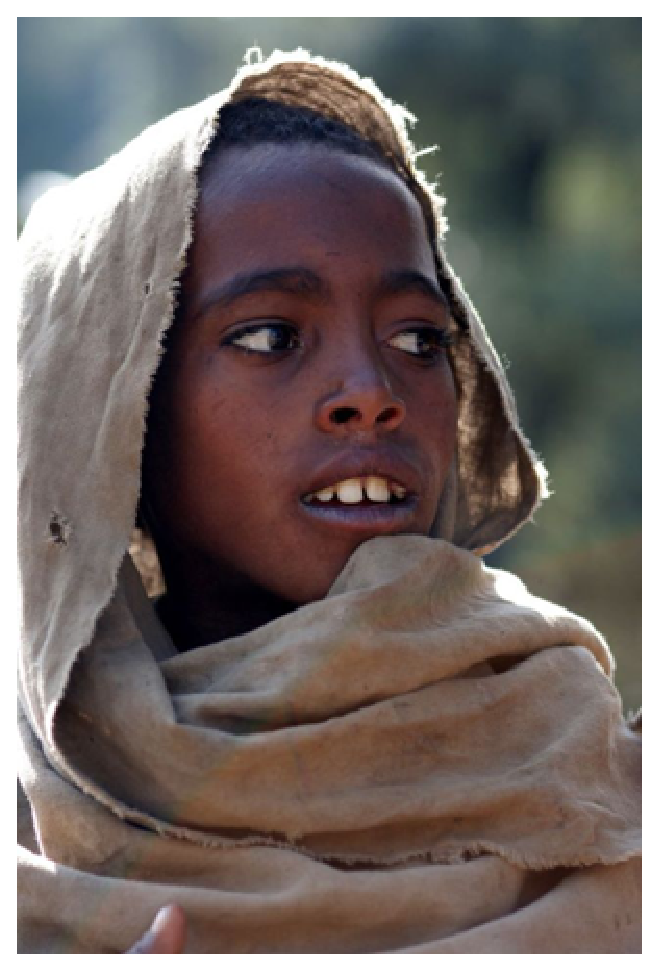
\includegraphics{etiopan.eps}
\reflectbox{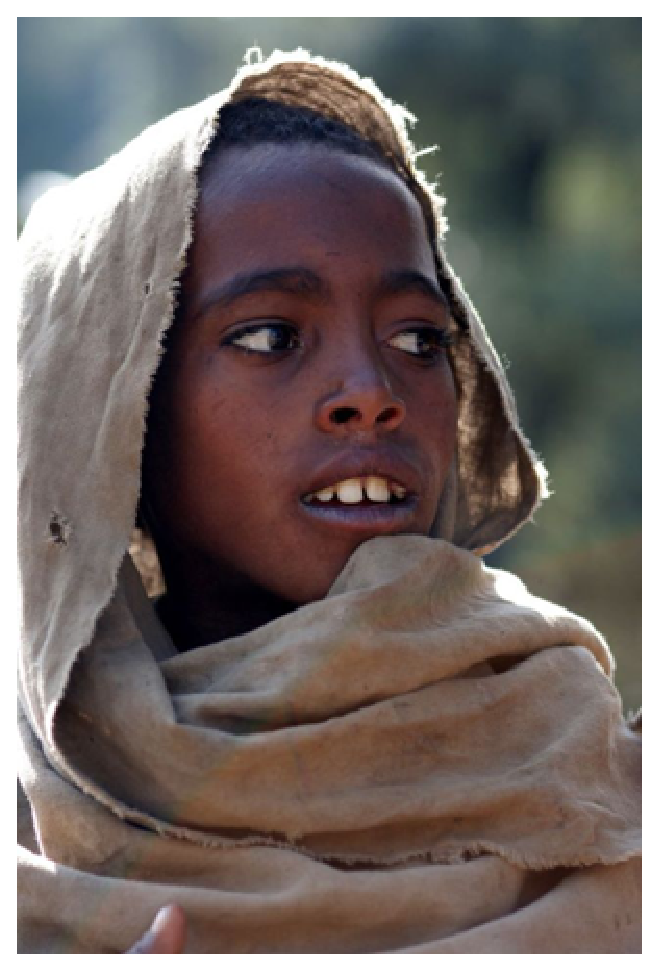
\includegraphics{etiopan.eps}}}
\begin{figure}[h]\caption{Malý etiopánek a jeho bratřícek}\end{figure}
\end{center}


Rozdíl medzi vektorovým \ldots

\begin{center}
\scalebox{0.4}{
\includegraphics{oniisan.eps}}
\begin{figure}[h]\caption{Vektorový obrázek}\end{figure}
\end{center}

\ldots a bitmapovým obrázkem

\begin{center}
\scalebox{0.6}{
\includegraphics{oniisan2.eps}}
\begin{figure}[h]\caption{Bitmapový obrázek}\end{figure}
\end{center}

se projeví například při zvětšení.

Odkazy (nejen ty) na obrázky 1,2 a 3, na tabulky 1 a 2 a také na algoritmus \ref{alg:one} jsou udělány pomocí křížových odkazů. Pak je ovšem potřeba zdrojový soubor přeložit dvakrát.

Vektorové obrázky lze vytvořit i přímo v {\LaTeX}u, například pomocí protředí \verb|picture|. Všechny rozměry jsou uváděny v mm.

\end{document}